% Colores
\definecolor{color1}{RGB}{0,255,0}
\definecolor{color2}{RGB}{255,165,0}
\definecolor{color3}{RGB}{128,0,128}
\definecolor{color4}{RGB}{128,128,0}
\definecolor{color5}{RGB}{0,128,128}
\definecolor{color6}{RGB}{128,0,128}
\def\rectasi{
  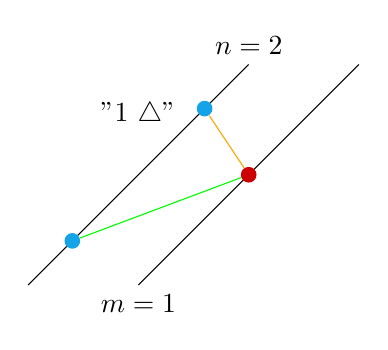
\begin{tikzpicture}[scale=0.7]

    \node at (2,3.1) {"1 $\triangle$"};
    % Draw the two parallel lines
    \draw (0,0) -- (4,4) node[above]{$n=2$};
    \draw (2,0) node[below]{$m=1$} -- (6,4) ;

    % Points on first line with nodes
    \foreach \y [count=\i] in {0.8,3.2} {
        \node[circle, fill=Cerulean, inner sep=2pt] (A\i) at (\y,\y) {};
      }

    % Points on second line with nodes
    \foreach \y [count=\i] in {2} {
        \node[circle, fill=red!80!black, inner sep=2pt] (B\i) at ({\y+2},\y) {};
      }

    % Connect all points between lines
    \foreach \i [count=\k] in {1,2} {
        \foreach \j in {1} {
            \draw[color=color\k, thin] (A\i) -- (B\j);
          }
      }
  \end{tikzpicture}
}

\def\rectasii{
  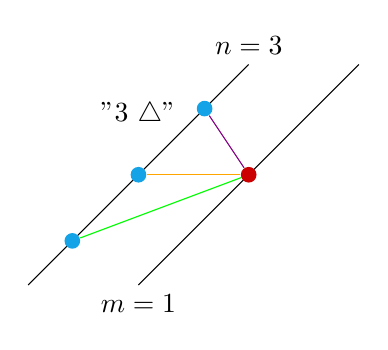
\begin{tikzpicture}[scale=0.7]

    \node at (2,3.1) {"3 $\triangle$"};
    % Draw the two parallel lines
    \draw (0,0) -- (4,4) node[above]{$n=3$};
    \draw (2,0) node[below]{$m=1$} -- (6,4) ;

    % Points on first line with nodes
    \foreach \y [count=\i] in {0.8,2,3.2} {
        \node[circle, fill=Cerulean, inner sep=2pt] (A\i) at (\y,\y) {};
      }

    % Points on second line with nodes
    \foreach \y [count=\i] in {2} {
        \node[circle, fill=red!80!black, inner sep=2pt] (B\i) at ({\y+2},\y) {};
      }

    % Connect all points between lines
    \foreach \i [count=\k] in {1,2,3} {
        \foreach \j in {1} {
            \draw[color=color\k, thin] (A\i) -- (B\j);
          }
      }
  \end{tikzpicture}
}

\def\rectasiii{
  \begin{tikzpicture}[scale=0.7]
    \node at (2,3.1) {"4 $\triangle$"};

    \draw (0,0) -- (4,4) node[above]{$n=2$};
    \draw (2,0) node[below]{$m=2$} -- (6,4) ;

    % Points on first line with nodes
    \foreach \y [count=\i] in {0.8,3.2} {
        \node[circle, fill=Cerulean, inner sep=2pt] (A\i) at (\y,\y) {};
      }

    % Points on second line with nodes
    \foreach \y [count=\i] in {0.8,3.2} {
        \node[circle, fill=red!80!black, inner sep=2pt] (B\i) at ({\y+2},\y) {};
      }

    % Connect all points between lines
    \foreach \i [count=\k] in {1,2,3} {
        \foreach \j in {1,2} {
            \draw[color=color\k, thin] (A\i) -- (B\j);
          }
      }
  \end{tikzpicture}
}

\def\rectasiv{
  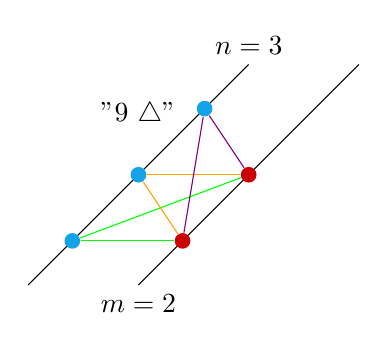
\begin{tikzpicture}[scale=0.7]
    \node at (2,3.1) {"9 $\triangle$"};

    \draw (0,0) -- (4,4) node[above]{$n=3$};
    \draw (2,0) node[below]{$m=2$} -- (6,4) ;

    % Points on first line with nodes
    \foreach \y [count=\i] in {0.8,2,3.2} {
        \node[circle, fill=Cerulean, inner sep=2pt] (A\i) at (\y,\y) {};
      }

    % Points on second line with nodes
    \foreach \y [count=\i] in {0.8,2} {
        \node[circle, fill=red!80!black, inner sep=2pt] (B\i) at ({\y+2},\y) {};
      }

    % Connect all points between lines
    \foreach \i [count=\k] in {1,2,3} {
        \foreach \j in {1,2} {
            \draw[color=color\k, thin] (A\i) -- (B\j);
          }
      }
  \end{tikzpicture}
}

\begin{enunciado}{\ejercicio}
  Dadas dos rectas paralelas en el plano, se marcan $n$ puntos distintos sobre una y $m$ puntos distintos sobre la otra.
  ¿Cuántos triángulos se pueden formar con vértices en esos puntos?
\end{enunciado}

Haciendo para algunos casos a mano se tiene algo así:
$$
  \rectasi \rectasii \rectasiii \rectasiv
$$
Para armar un triángulo con 3 vértices \href{\mindExplosion}{\faIcon[regular]{meh-rolling-eyes}},
tengo que agarrar 1 vértice de una recta y 2 vértices de la otra.

\begin{enumerate}[label=(\Roman*)]
  \item
        Agarro \blue{1} de la recta que tiene $n$ y {\color{red!80!black}2} de la que tiene $m$.
        \begin{center}
          De la primera tengo $n$ opciones y agarro 1. Cantidad de formas de hacer eso: $\binom{n}{1}$

          De la segunda tengo $m$ opciones y agarro 2. Cantidad de formas de hacer eso: $\binom{m}{2}$
        \end{center}

        Es decir que tengo:
        $$
          \binom{n}{1}
          \binom{m}{2}
          = \frac{n \cdot m \cdot (m - 1)}{2}
        $$

  \item
        Parecido pero cambiando las rectas, agarrando ahora {\color{red!80!black}1} de la que tiene $m$ y
        \blue{2} de la que tiene $n$:
        \begin{center}
          De la primera tengo $m$ opciones y agarro 1. Cantidad de formas de hacer eso: $\binom{m}{1}$

          De la segunda tengo $n$ opciones y agarro 2. Cantidad de formas de hacer eso: $\binom{n}{2}$
        \end{center}

        Es decir que tengo:
        $$
          \binom{m}{1}
          \binom{n}{2}
          = \frac{m \cdot n \cdot (n - 1)}{2}
        $$

        \bigskip

        Finalmente sumo lo encontrado. La cantidad total de triángulos será:
        $$
          \frac{n \cdot m \cdot (m - 1)}{2}
          +
          \frac{m \cdot n \cdot (n - 1)}{2}
          =
          \cajaResultado{
            \frac{n \cdot m \cdot (n + m - 2)}{2}
          }
        $$
\end{enumerate}

\begin{aportes}
  \item \aporte{\dirRepo}{naD GarRaz \github}
  \item \aporte{\neverGonnaGiveYouUp}{Malena \youtube}
\end{aportes}
